\documentclass[a4paper,12pt]{article}
\usepackage[utf8]{inputenc}
\usepackage[english]{babel}
\usepackage{graphicx}
\usepackage{geometry}
\usepackage{listings}
\usepackage{xcolor}
\usepackage{tikz}
\usetikzlibrary{shapes, arrows, positioning}

\geometry{top=2cm, bottom=2cm, left=2.5cm, right=2.5cm}

\definecolor{codegray}{rgb}{0.5,0.5,0.5}
\definecolor{backcolour}{rgb}{0.95,0.95,0.92}

\lstdefinestyle{mystyle}{
    backgroundcolor=\color{backcolour},   
    commentstyle=\color{codegray},
    keywordstyle=\color{blue},
    basicstyle=\ttfamily\footnotesize,
    breakatwhitespace=false,         
    breaklines=true,                 
    captionpos=b,                    
    keepspaces=true,              
    numbers=left,                    
    numbersep=5pt,                  
    showspaces=false,                
    showstringspaces=false,
    showtabs=false,                  
    tabsize=2,
    frame=single
}
\lstset{style=mystyle}

\title{\textbf{Practical Work 3: MPI File Transfer}}
\author{Group ID: 16}
\date{\today}

\begin{document}

\maketitle

\section{Introduction}
The objective of this practical work is to upgrade a standard file transfer system into a distributed version using the Message Passing Interface (MPI). The system allows a file to be transferred from a sender process to a receiver process running in parallel.

\section{Implementation Choice}
We selected Python and the mpi4py library for this project. This choice allows us to leverage Python's simplicity for file I/O operations while utilizing the robust MPI standard bindings provided by mpi4py for process communication. It supports sending both serialized Python objects (for metadata) and binary buffers (for file content).

\section{System Design}

\subsection{Architecture}
The system adopts a master-slave communication model where Rank 0 acts as the Sender and Rank 1 acts as the Receiver.

\begin{figure}[h]
    \centering
    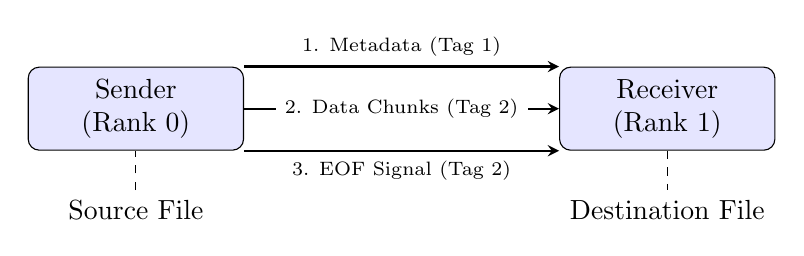
\begin{tikzpicture}[
        node distance=3cm,
        process/.style={rectangle, draw, fill=blue!10, text width=2.5cm, text centered, rounded corners, minimum height=3em},
        arrow/.style={thick,->,>=stealth}
    ]
    
    \node [process] (sender) {Sender (Rank 0)};
    \node [process, right=4cm of sender] (receiver) {Receiver (Rank 1)};
    
    \node [below=0.5cm of sender] (file1) {Source File};
    \node [below=0.5cm of receiver] (file2) {Destination File};
    
    \draw [dashed] (file1) -- (sender);
    \draw [dashed] (receiver) -- (file2);
    
    \draw [arrow] (sender.north east) -- node[above, font=\scriptsize] {1. Metadata (Tag 1)} (receiver.north west);
    \draw [arrow] (sender.east) -- node[fill=white, font=\scriptsize] {2. Data Chunks (Tag 2)} (receiver.west);
    \draw [arrow] (sender.south east) -- node[below, font=\scriptsize] {3. EOF Signal (Tag 2)} (receiver.south west);

    \end{tikzpicture}
    \caption{Data Flow Diagram}
\end{figure}

\section{Implementation Details}

\subsection{Sender Logic}
The sender reads the file and transmits it in chunks.

\begin{lstlisting}[language=Python]
def sender(self, filename):
    size = os.path.getsize(filename)
    self.comm.send({'filename': filename, 'filesize': size}, dest=1, tag=1)

    with open(filename, 'rb') as f:
        while True:
            chunk = f.read(self.buffer_size)
            if not chunk: break
            self.comm.send(chunk, dest=1, tag=2)
    
    self.comm.send(None, dest=1, tag=2)
\end{lstlisting}

\subsection{Receiver Logic}
The receiver listens for metadata and then loops to receive content chunks.

\begin{lstlisting}[language=Python]
def receiver(self):
    meta = self.comm.recv(source=0, tag=1)
    new_name = "received_" + meta['filename']

    with open(new_name, 'wb') as f:
        while True:
            chunk = self.comm.recv(source=0, tag=2)
            if chunk is None: break
            f.write(chunk)
\end{lstlisting}

\section{Roles and Responsibilities}
\begin{table}[h]
\centering
\begin{tabular}{|l|l|p{6cm}|}
\hline
\textbf{Member} & \textbf{Role} & \textbf{Tasks} \\ \hline
Member 1 & Architect & Designed the communication protocol and data flow. \\ \hline
Member 2 & Developer & Implemented the file I/O and MPI logic. \\ \hline
Member 3 & Analyst & Verified the file integrity and wrote the report. \\ \hline
\end{tabular}
\caption{Group Task Allocation}
\end{table}

\end{document}